\documentclass[nofootinbib,superscriptaddress,a4paper,twocolumn,longbibliography,floatfix,pra]{revtex4-2}
\usepackage[english]{babel}
\usepackage[utf8]{inputenc}

\usepackage{enumitem}

\usepackage{amsfonts}
\usepackage{amsthm}
\usepackage{mathtools}
\usepackage{physics}
\usepackage{xcolor}
\usepackage{graphicx}
\usepackage[left=23mm,right=13mm,top=35mm,columnsep=15pt]{geometry} 
\usepackage{adjustbox}
\usepackage{placeins}
\usepackage[T1]{fontenc}
\usepackage{lipsum}
\usepackage{csquotes}

\usepackage{listings}
\usepackage{xcolor}

\definecolor{codegreen}{rgb}{0,0.6,0}
\definecolor{codegray}{rgb}{0.5,0.5,0.5}
\definecolor{codepurple}{rgb}{0.58,0,0.82}
\definecolor{tqblue}{HTML}{08293d}
\definecolor{backcolour}{HTML}{fefdf5}

\lstdefinestyle{mystyle}{
    backgroundcolor=\color{backcolour},   
    commentstyle=\color{codegreen},
    keywordstyle=\color{magenta},
    numberstyle=\tiny\color{codegray},
    stringstyle=\color{codepurple},
    basicstyle=\ttfamily\footnotesize\color{tqblue},
    breakatwhitespace=false,         
    breaklines=true,
    postbreak=\mbox{\textcolor{magenta}{$\hookrightarrow$}\space},                 
    captionpos=b,                    
    keepspaces=true,                 
    numbers=left,                    
    numbersep=5pt,                  
    showspaces=false,                
    showstringspaces=false,
    showtabs=false,                  
    tabsize=2
}

\lstset{style=mystyle}

\usepackage{booktabs}
\usepackage{soul}

\usepackage{xspace}
\newcommand{\expect}[2]{\ensuremath{\langle #1 \rangle_{#2}}}

\setlength{\parindent}{0cm}

\usepackage[pdftex, pdftitle={Article}, pdfauthor={Author}]{hyperref} % For hyperlinks in the PDF
\usepackage{xcolor}
\hypersetup{
    colorlinks,
    linkcolor={red!50!black},
    citecolor={blue!50!black},
    urlcolor={blue!80!black}
}

%-----------------------------------------------------------------------------%
% Macros:
%-----------------------------------------------------------------------------%

\newcommand{\comment}[1]{\begin{quote}\sf 
    \textcolor{blue}{[#1]}\end{quote}}
\newcommand{\linecomment}[1]{\textcolor{blue}{\sf[#1]}}

\newcommand{\tinyspace}{\mspace{1mu}}
\newcommand{\microspace}{\mspace{0.5mu}}
\newcommand{\negsmallspace}{\mspace{-1.5mu}}
\newcommand{\pt}{\operatorname{T}}
\newcommand{\ppt}{\operatorname{PPT}}
\newcommand{\sep}{\operatorname{Sep}}
\renewcommand{\int}{\operatorname{int}}
\renewcommand{\det}{\operatorname{Det}}
\renewcommand{\vec}{\operatorname{vec}}
\newcommand{\fid}{\operatorname{F}}
\newcommand{\im}{\operatorname{im}}

\renewcommand{\tr}{\operatorname{Tr}}
\renewcommand{\t}{{\scriptscriptstyle\mathsf{T}}}

\renewcommand{\abs}[1]{\lvert #1 \rvert}
\newcommand{\bigabs}[1]{\bigl\lvert #1 \bigr\rvert}
\newcommand{\Bigabs}[1]{\Bigl\lvert #1 \Bigr\rvert}
\newcommand{\biggabs}[1]{\biggl\lvert #1 \biggr\rvert}
\newcommand{\Biggabs}[1]{\Biggl\lvert #1 \Biggr\rvert}

\renewcommand{\ip}[2]{\langle #1 , #2\rangle}
\newcommand{\bigip}[2]{\bigl\langle #1, #2 \bigr\rangle}
\newcommand{\Bigip}[2]{\Bigl\langle #1, #2 \Bigr\rangle}
\newcommand{\biggip}[2]{\biggl\langle #1, #2 \biggr\rangle}
\newcommand{\Biggip}[2]{\Biggl\langle #1, #2 \Biggr\rangle}

\newcommand{\ceil}[1]{\lceil #1 \rceil}
\newcommand{\bigceil}[1]{\bigl\lceil #1 \bigr\rceil}
\newcommand{\Bigceil}[1]{\Bigl\lceil #1 \Bigr\rceil}
\newcommand{\biggceil}[1]{\biggl\lceil #1 \biggr\rceil}
\newcommand{\Biggceil}[1]{\Biggl\lceil #1 \Biggr\rceil}

\newcommand{\floor}[1]{\lfloor #1 \rfloor}
\newcommand{\bigfloor}[1]{\bigl\lfloor #1 \bigr\rfloor}
\newcommand{\Bigfloor}[1]{\Bigl\lfloor #1 \Bigr\rfloor}
\newcommand{\biggfloor}[1]{\biggl\lfloor #1 \biggr\rfloor}
\newcommand{\Biggfloor}[1]{\Biggl\lfloor #1 \Biggr\rfloor}

\newcommand{\bignorm}[1]{\bigl\lVert\tinyspace #1 \tinyspace\bigr\rVert}
\newcommand{\Bignorm}[1]{\Bigl\lVert\tinyspace #1 \tinyspace\Bigr\rVert}
\newcommand{\biggnorm}[1]{\biggl\lVert\tinyspace #1 \tinyspace\biggr\rVert}
\newcommand{\Biggnorm}[1]{\Biggl\lVert\tinyspace #1 \tinyspace\Biggr\rVert}

\newcommand{\bigtriplenorm}[1]{
  \bigl\lvert\!\microspace\bigl\lvert\!\microspace\bigl\lvert #1 
  \bigr\rvert\!\microspace\bigr\rvert\!\microspace\bigr\rvert}

\newcommand{\Bigtriplenorm}[1]{
  \Bigl\lvert\!\microspace\Bigl\lvert\!\microspace\Bigl\lvert #1 
  \Bigr\rvert\!\microspace\Bigr\rvert\!\microspace\Bigr\rvert}

\newcommand{\biggtriplenorm}[1]{
  \biggl\lvert\!\microspace\biggl\lvert\!\microspace\biggl\lvert #1 
  \biggr\rvert\!\microspace\biggr\rvert\!\microspace\biggr\rvert}

\newcommand{\Biggtriplenorm}[1]{
  \Biggl\lvert\!\microspace\Biggl\lvert\!\microspace\Biggl\lvert #1 
  \Biggr\rvert\!\microspace\Biggr\rvert\!\microspace\Biggr\rvert}

\newcommand{\triplenorm}[1]{
  \left\lvert\!\microspace\left\lvert\!\microspace\left\lvert #1 
  \right\rvert\!\microspace\right\rvert\!\microspace\right\rvert}
\def\iso{\cong}
\newcommand{\defeq}{\triangleq}

\newcommand{\bigket}[1]{
  \bigl\lvert\microspace #1 \microspace \bigr\rangle}

\newcommand{\Bigket}[1]{
  \Bigl\lvert\microspace #1 \microspace \Bigr\rangle}

\newcommand{\biggket}[1]{
  \biggl\lvert\microspace #1 \microspace \biggr\rangle}

\newcommand{\Biggket}[1]{
  \Biggl\lvert\microspace #1 \microspace \Biggr\rangle}

\newcommand{\bigbra}[1]{
  \bigl\langle\microspace #1 \microspace \bigr\rvert}

\newcommand{\Bigbra}[1]{
  \Bigl\langle\microspace #1 \microspace \Bigr\rvert}

\newcommand{\biggbra}[1]{
  \biggl\langle\microspace #1 \microspace \biggr\rvert}

\newcommand{\Biggbra}[1]{
  \Biggl\langle\microspace #1 \microspace \Biggr\rvert}

\newcommand{\I}{\mathbb{I}}

\newcommand{\setft}[1]{\mathrm{#1}}
\newcommand{\Density}{\setft{D}}
\newcommand{\Pos}{\setft{Pos}}
\newcommand{\Unitary}{\setft{U}}
\newcommand{\Herm}{\setft{Herm}}
\newcommand{\Lin}{\setft{L}}

\newcommand{\complex}{\mathbb{C}}
\renewcommand{\natural}{\mathbb{N}}
\newcommand{\integer}{\mathbb{Z}}

\usepackage{FiraSans}
\newcommand{\poly}{\mathit{poly}}
\newcommand{\toqitofont}{%
	\fontfamily{FiraSans}%
	\selectfont}


\newcommand{\toqito}{ $|${\toqitofont toqito}$\rangle$\xspace}
\newcommand{\numpy}{\texttt{numpy}\xspace}
\newcommand{\tequila}{\textsc{toqito}}
\newenvironment{mylist}[1]{\begin{list}{}{
	\setlength{\leftmargin}{#1}
	\setlength{\rightmargin}{0mm}
	\setlength{\labelsep}{2mm}
	\setlength{\labelwidth}{8mm}
	\setlength{\itemsep}{0mm}}}
	{\end{list}}

\newenvironment{namedtheorem}[1]
	       {\begin{trivlist}\item {\bf #1.}\em}{\end{trivlist}}

\newcommand{\X}{\mathcal{X}}
\newcommand{\Y}{\mathcal{Y}}
\newcommand{\Z}{\mathcal{Z}}
\newcommand{\W}{\mathcal{W}}
\newcommand{\A}{\mathcal{A}}
\newcommand{\B}{\mathcal{B}}
\newcommand{\V}{\mathcal{V}}
\newcommand{\U}{\mathcal{U}}
\newcommand{\C}{\mathcal{C}}
\newcommand{\D}{\mathcal{D}}
\newcommand{\E}{\mathcal{E}}
\newcommand{\F}{\mathcal{F}}
\newcommand{\M}{\mathcal{M}}
\newcommand{\N}{\mathcal{N}}
\newcommand{\R}{\mathcal{R}}
\newcommand{\Q}{\mathcal{Q}}
\renewcommand{\P}{\mathcal{P}}
\renewcommand{\S}{\mathcal{S}}
\newcommand{\T}{\mathcal{T}}
\newcommand{\K}{\mathcal{K}}
\renewcommand{\L}{\mathcal{L}}

\newcommand{\yes}{\text{yes}}
\newcommand{\no}{\text{no}}

\newcommand{\class}[1]{\textup{#1}}
\newcommand{\reg}[1]{\textsf{#1}}

\def\BB84{\mathsf{BB84}}
\def\CHSH{\mathsf{CHSH}}
\def\MUB{\mathsf{MUB}}

\begin{document}
\title{\toqito: Theory of quantum information toolkit}

\author{Vincent Russo}
\email[E-mail:]{vincentrusso1@gmail.com}
\affiliation{-}

\date{\today}

\begin{abstract}
    \toqito is an open source Python library for studying various objects in
    quantum information, namely, states, channels, and measurements. \toqito
    focuses on providing numerical tools to study problems pertaining to
    entanglement theory, nonlocal games, and other aspects of quantum
    information that are often associated with computer science. We illustrate
    some of the core features of \toqito and show how it can be applied to
    certain problems in quantum information. Using \toqito, we provide an
    answer to one of the problems left open in~\cite{johnston2016extended} by
    showing a more minimal example of an extended nonlocal game that possesses
    a quantum advantage. We also make use of \toqito to numerically verify a
    number of known results in the literature on subjects including quantum
    state discrimination and nonlocal games. We hope that these numerical tools
    can be used to aid researchers in further investigating these areas as well
    as students studying quantum information.
\end{abstract}

\maketitle

%-----------------------------------------------------------------------------%
\section{Introduction}
\label{sec:introduction}
%-----------------------------------------------------------------------------%

\comment{Intro}

While there are many software packages that exist in the quantum software
ecosystem, few of them have a core focus on quantum information.  Packages such
as XX and XX specialize in quantum circuit synthesis and packages XX, XX, and
XX center on problems pertaining to quantum machine learning~\cite{}. Software
packages with a focus on quantum information .... For a more thorough survey on
software packages pertaining to quantum information, consult the following
survey~\cite{}. 

\toqito is an ... Documentation and tutorials are available on the \toqito
\href{https://github.com/vprusso/toqito}{GitHub repository}~\cite{toqito}.


%-----------------------------------------------------------------------------%
\section{Fundamental objects}
\label{sec:fundemental_objects}
%-----------------------------------------------------------------------------%

Arguably, the core building blocks of quantum information consist of
\emph{states}, \emph{channels}, and \emph{measurements}.\\

\subsection{States}\label{sec:states}

A \emph{quantum state} is a density operator
\begin{equation}
    \rho \in \Density(\X)
\end{equation}
where $\X$ is a complex Euclidean space and where $\Density(\cdot)$ represents
the set of density matrices, that is, the set of matrices that are positive
semidefinite with trace equal to $1$.

%-----------------------------------------------------------------------------%
\subsection{Measurements}
\label{sec:measurements}
%-----------------------------------------------------------------------------%

A \emph{measurement} can be defined as a function
\begin{equation}
    \mu: \Sigma \rightarrow \Pos(\X)
\end{equation}
satisfying
\begin{equation}
    \sum_{a \in \Sigma} \mu(a) = \I_{\X}
\end{equation}
where $\Sigma$ represents a set of measurement outcomes and where $\mu(a)$
represents the measurement operator associated with outcome $a \in \Sigma$.

%-----------------------------------------------------------------------------%
\section{Examples and Applications}
\label{sec:examples_and_applications}
%-----------------------------------------------------------------------------%

The \toqito software package \comment{TODO: elaborate}

%-----------------------------------------------------------------------------%
\subsection{Nonlocal games}\label{sec:nonlocal_games}
%-----------------------------------------------------------------------------%

In this section, we are going to cover the notion of a \emph{nonlocal game}; a
mathematical framework that abstractly models a physical system. The simplest
instance of a nonlocal game involves two players--Alice and Bob, who are not
allowed to communicate with each other once the game has started and who play
cooperatively against an adversary referred to as the referee. \\

A primary challenge that arises when studying these games is to determine the
maximum probability with which Alice and Bob are able to achieve a winning
outcome. \\

The probability is dependent on the type of \emph{strategy} that Alice and Bob
use in the game. A \emph{classical strategy} is one in which Alice and Bob have
access to classical resources and play deterministically. The best that Alice
and Bob can do using a classical strategy is known as the \emph{classical
value} of the game.  Similarly, a \emph{quantum strategy} is one in which Alice
and Bob have access to quantum resources in the form of a shared quantum state
and respective sets of measurements. The best that Alice and Bob can do using a
quantum strategy is known as the \emph{quantum value} of the game.
\\

\begin{figure}[!htpb]
    \centering
    \includegraphics[width=0.4\textwidth]{pics/nonlocal_game_quantum_strategy.pdf}
    \caption{A nonlocal game}
    \label{fig:nonlocal_game}
\end{figure}

More formally, a nonlocal game, $G$, is specified as a pair $(\pi, V)$ where
$\pi$ is a probability distribution
\begin{equation}
    \pi : \Sigma_A \times \Sigma_B \rightarrow [0,1]
\end{equation}
on the Cartesian product of two alphabets $\Sigma_A$ and $\Sigma_B$, and $V$ is
a function
\begin{equation}
    V : \Gamma_A \times \Gamma_B \times \Sigma_A \times \Sigma_B \rightarrow [0,1].
\end{equation}
We shall represent
\begin{equation}
    \Sigma = \Sigma_A \times \Sigma_B 
    \ \ \text{and} \ \ 
    \Gamma = \Gamma_A \times \Gamma_B
\end{equation}
to denote the respective sets of questions and answers for Alice and Bob.


%-----------------------------------------------------------------------------%
\subsubsection{Classical strategies for nonlocal games}
\label{sec:classical_strategies_for_nonlocal_games}
%-----------------------------------------------------------------------------%

%-----------------------------------------------------------------------------%
\subsubsection{Quantum strategies for nonlocal games}
\label{sec:quantum_strategies_for_nonlocal_games}
%-----------------------------------------------------------------------------%

%-----------------------------------------------------------------------------%
\subsubsection{Non-signaling strategies for nonlocal games}
\label{sec:non_signaling_strategies_for_nonlocal_games}
%-----------------------------------------------------------------------------%

%-----------------------------------------------------------------------------%
\subsubsection{Parallel repetition for nonlocal games}
\label{sec:parallel_repeptitionfor_nonlocal_games}
%-----------------------------------------------------------------------------%

A game $G$ has the property of \emph{strong parallel repetition} if the value
of the game raised to the power $r$ is equal to the value of running the game
$r$ times.

%-----------------------------------------------------------------------------%
\subsection{XOR nonlocal games}
\label{sec:xor_nonlocal_games}
%-----------------------------------------------------------------------------%

A \emph{two-player XOR nonlocal game} is a nonlocal game in which the winning
condition is predicated on an XOR function~\cite{cleve2004consequences}.

%-----------------------------------------------------------------------------%
\subsubsection{Example: The CHSH game}
\label{sec:chsh_game}
%-----------------------------------------------------------------------------%

The \emph{CHSH game} is a two-player XOR game with the following probability
distribution 
\begin{equation}
    \pi(x,y) = \frac{1}{4},
\end{equation}
and question and answer sets
\begin{equation}
    \begin{aligned}
        (x,y) \in \Sigma_A \times \Sigma_B \quad \text{and} \quad (a,b) \in
        \Gamma_A \times \Gamma_B,
    \end{aligned}
\end{equation}
where 
\begin{equation}
    \Sigma_A = \Sigma_B = \Gamma_A = \Gamma_B = \{0,1\}.
\end{equation}
Alice and Bob win the CHSH game if and only if the following equation is
satisfied
\begin{equation}
    a \oplus b = x \land y.
\end{equation}
For each question scenario, Table~\ref{tab:chsh_winning} provides what the
winning condition must be equal to for each question tuple to induce a winning
outcome.
\begin{table}[!htpb]\label{tab:chsh_winning}
    \begin{tabular}{|c|c|c|}
        \hline
        \textbf{$x$} & \textbf{$y$} & \textbf{$a \oplus b$} \\ \hline
        0 & 0 & 0 \\ \hline
        0 & 1 & 0 \\ \hline
        1 & 0 & 0 \\ \hline
        1 & 1 & 1 \\ \hline
    \end{tabular}
    \caption{Question pairs and respective winning outcomes for the CHSH game.}
\end{table}
In order to specify an XOR nonlocal game in \toqito, we will define two
matrices:

\begin{itemize}[noitemsep]
    \item \texttt{prob\_mat}: A matrix whose $(x,y)^{th}$-entry corresponds to
        the probability that Alice receives question $x$ and Bob receives
        question $y$. \\
    \item \texttt{pred\_mat}: A matrix whose $(x,y)^{th}$-entry corresponds to
        the winning choice of $a$ and $b$ when Alice receives $x$ and Bob
        receives $y$ from the referee.
\end{itemize}

We can encode the CHSH game, $G_{\CHSH} = (\pi, V)$, in \toqito by defining the
\texttt{prob\_mat} and \texttt{pred\_mat} variables as is shown in
Figure~\ref{fig:chsh}.

\begin{figure}[!htpb]
    \centering
    \lstinputlisting[language=Python]{code/chsh.py}        
    \caption{Define the CHSH XOR nonlocal game.}
    \label{fig:chsh}
\end{figure}

That is, the \texttt{prob\_mat} variable encapsulates that each question pair
$\{(0,0),(0,1),(1,0),(1,1)\}$ is equally likely. The \texttt{pred\_mat}
variable indicates what the winning outcome of Alice and Bob should be. For
instance, \texttt{pred\_mat[0][0] = 0} describes the scenario where Alice and
Bob both receive $0$ as input. As we want to satisfy the winning condition $a
\oplus b = x \land y$, we must have that $a \oplus b = 0$ to satisfy the case
when both $x$ and $y$ are equal to zero. A similar logic can be followed to
populate the remaining entries of the \texttt{pred\_mat} variable.

What is very intriguing about the CHSH game is that it is an example of a
nonlocal game where the players can do \emph{strictly} better if they make use
of a quantum strategy instead of a classical one. It is known that the best
that Alice and Bob can do when using a classical strategy is to win $G_{\CHSH}$
with probability $3/4$, however, there exists a quantum strategy that enables
Alice and Bob to win with a strictly higher probability of $\cos^2(\pi/8)
\approx 0.8536$~\cite{cleve2004consequences}. We can numerically verify this
fact in \toqito as is shown in Figure~\ref{fig:chsh_classical_quantum}

\begin{figure}[!htpb]
    \centering
    \lstinputlisting[language=Python]{code/chsh_classical_quantum.py}        
    \caption{Calculate the classical and quantum value of the CHSH XOR nonlocal
    game.}
    \label{fig:chsh_classical_quantum}
\end{figure}

Using \toqito, we can also compute how a given XOR nonlocal game behaves under
parallel repetition. It holds from~\cite{cleve2008perfect} that the quantum
value of any XOR nonlocal game obeys strong parallel repetition. That is, it
holds that 

\begin{equation}
    \omega^*(G^n) = \omega^*(G)^n 
\end{equation} 

for any XOR nonlocal game, $G$. The \texttt{XORGame} class takes an optional
argument, \texttt{reps}, that specifies how many parallel repetitions to run
the game for (by default, this argument is equal to one). For instance, taking
the \texttt{prob\_mat} and \texttt{pred\_mat} variables defined in
Figure~\ref{fig:chsh} that characterize $G_{\CHSH}$, we can consider the value
of the $r$-fold parallel repetition of $G_{\CHSH}$.
Figure~\ref{fig:chsh_parallel_repetition} illustrates how one may compute the
$2$-fold and $3$-fold parallel repetition of the CHSH game for the quantum
value.

\begin{figure}[!htpb]
    \centering
    \lstinputlisting[language=Python]{code/chsh_parallel_repetition.py}        
    \caption{Calculate $2$-fold and $3$-fold parallel repetition of the CHSH game.}
    \label{fig:chsh_parallel_repetition}
\end{figure}





%-----------------------------------------------------------------------------%
\subsection{Extended nonlocal games}
\label{sec:extended_nonlocal_games}
%-----------------------------------------------------------------------------%

In this section we shall define the concept of an \emph{extended nonlocal
game}. Extended nonlocal games are a more general abstraction of nonlocal games
wherein the referee, who previously only provided questions and answers to the
players, now shares a state with the players and is able to perform a
measurement on that shared state.
\\

Every extended nonlocal game has a \emph{value} associated to it. Analogously
to nonlocal games, this value is a quantity that dictates how well the players
can perform a task in the extended nonlocal game model when given access to
certain resources. We will be using \toqito to calculate these quantities.
\\

Extended nonlocal games have a natural physical interpretation in the setting
of tripartite steering~\cite{cavalcanti2015detection} and in device-independent
quantum scenarios~\cite{tomamichel2013monogamy}, For more information on
extended nonlocal games, please refer to~\cite{johnston2016extended,
russo2017extended, russo2017thesis}.

%-----------------------------------------------------------------------------%
\subsubsection{The extended nonlocal game model}
\label{sec:extended_nonlocal_game_model}
%-----------------------------------------------------------------------------%

An extended nonlocal game is similar to a nonlocal game in the sense that it is
a cooperative game played between two players Alice and Bob against a referee.
The game begins much like a nonlocal game, with the referee selecting and
sending a pair of questions $(x,y)$ according to a fixed probability
distribution. Once Alice and Bob receive $x$ and $y$, they respond with
respective answers $a$ and $b$. Unlike a nonlocal game, the outcome of an
extended nonlocal game is determined by measurements performed by the referee
on its share of the state initially provided to it by Alice and Bob.

\begin{figure}[!htpb]
    \centering
    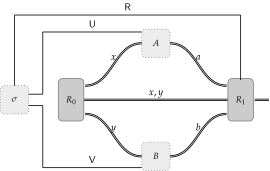
\includegraphics[width=0.4\textwidth]{pics/extended_nonlocal_game.pdf}
    \caption{An extended nonlocal game}
    \label{fig:extended_nonlocal_game}
\end{figure}

Specifically, Alice and Bob's winning probability is determined by collections
of measurements, $V(a,b|x,y) \in \Pos(\R)$, where $\R = \complex^m$ is a
complex Euclidean space with $m$ denoting the dimension of the referee's
quantum system--so if Alice and bob's response $(a,b)$ to the question pair
$(x,y)$ leaves the referee's system in the quantum state
\begin{equation}
    \sigma_{a,b}^{x,y} \in \Density(\R),
\end{equation}
then their winning and losing probabilities are given by
\begin{equation}
    \ip{V(a,b|x,y)}{\sigma_{a,b}^{x,y}} \quad \text{and} \quad \ip{\I -
    V(a,b|x,y)}{\sigma_{a,b}^{x,y}}.
\end{equation}

%-----------------------------------------------------------------------------%
\subsubsection{Strategies for extended nonlocal games}
\label{sec:strategies_for_extended_nonlocal_games}
%-----------------------------------------------------------------------------%

An extended nonlocal game $G$ is defined by a pair $(\pi, V)$, where $\pi$ is a
probability distribution of the form
\begin{equation}
    \pi: \Sigma_A \times \Sigma_B \rightarrow \left[0, 1\right]
\end{equation}
on the Cartesian product of two alphabets $\Sigma_A$ and $\Sigma_B$, and $V$ is
a function of the form
\begin{equation}
    V: \Gamma_A \times \Gamma_B \times \Sigma_A \times \Sigma_B \rightarrow
    \Pos(\R)
\end{equation}
for $\Sigma_A$ and $\Sigma_B$ as above, $\Gamma_A$ and $\Gamma_B$ being
alphabets, and $\R$ refers to the referee's space. Just as in the case for
nonlocal games, we shall use the convention that
\begin{equation}
    \Sigma = \Sigma_A \times \Sigma_B \quad \text{and} \quad \Gamma = \Gamma_A
    \times \Gamma_B
\end{equation}
to denote the respective sets of questions asked to Alice and Bob and the sets
of answers sent from Alice and Bob to the referee.

When analyzing a strategy for Alice and Bob, it may be convenient to define a
function
\begin{equation}
    K: \Gamma_A \times \Gamma_B \times \Sigma_A \times \Sigma_B \rightarrow
    \Pos(\R).
\end{equation}
We can represent Alice and Bob's winning probability for an extended nonlocal game as
\begin{equation}
    \sum_{(x,y) \in \Sigma} \pi(x,y) \sum_{(a,b) \in \Gamma}
    \ip{V(a,b|x,y)}{K(a,b|x,y)}.
\end{equation}

%-----------------------------------------------------------------------------%
\subsubsection{The BB84 extended nonlocal game}
%-----------------------------------------------------------------------------%

The \emph{BB84 extended nonlocal game} is defined as follows. Let $\Sigma_A =
\Sigma_B = \Gamma_A = \Gamma_B = \{0,1\}$, define
\begin{equation}
    \begin{aligned}
        V(0,0|0,0) = 
        \begin{pmatrix} 1 & 0 \\ 0 & 0 \end{pmatrix}, &\quad
        V(0,0|1,1) = 
        \frac{1}{2} \begin{pmatrix} 1 & 1 \\ 1 & 1 \end{pmatrix}, \\
        V(1,1|0,0) = 
        \begin{pmatrix} 0 & 0 \\ 0 & 1 \end{pmatrix}, &\quad
        V(1,1|1,1) = 
        \frac{1}{2} \begin{pmatrix} 1 & -1 \\ -1 & 1\end{pmatrix}
    \end{aligned}
\end{equation}
define
\begin{equation}
    V(a,b|x,y) = \begin{pmatrix} 0 & 0 \\ 0 & 0 \end{pmatrix}
\end{equation}
for all $a \not= b$ or $x \not= y$, define $\pi(0, 0) = \pi(1, 1) =
\frac{1}{2}$, and define $\pi(x,y) = 0$ if $x \not= y$.

We can encode the BB84 extended nonlocal game, $G_{\BB84} = (\pi, V)$, in
\numpy arrays where \texttt{prob\_mat} corresponds to the probability
distribution $\pi$ and where \texttt{pred\_mat} corresponds to the operator
$V$.

\begin{figure}[!htpb]
    \centering
    \lstinputlisting[language=Python]{code/bb84_game.py}        
    \caption{Define the BB84 extended nonlocal game.}
    \label{fig:bb84_game}
\end{figure}

In the following sections, we will use the BB84 extended nonlocal game as an
example for how one can define and compute the values of an extended nonlocal
game in \toqito.

%-----------------------------------------------------------------------------%
\subsubsection{Standard quantum strategies for extended nonlocal games}
\label{sec:standard_quantum_strategies_for_extended_nonlocal_games}
%-----------------------------------------------------------------------------%

A \emph{standard quantum strategy} for an extended nonlocal game consists of
finite-dimensional complex Euclidean spaces $\U$ for Alice and $\V$ for Bob, a
quantum state $\sigma \in \Density(\U \otimes \R \otimes \V)$ and two
collections of measurements
\begin{equation*}
    \{A_a^x : a \in \Gamma_A\} \subset \Pos(\U)
    \ \ \text{and} \ \
    \{B_b^y : b \in \Gamma_B\} \subset \Pos(\V),
\end{equation*}
for each $x \in \Sigma_A$ and $y \in \Sigma_B$. The winning probability for
such a strategy in this game $G = (\pi, V)$ is given by
\begin{equation}
    \sum_{(x,y) \in \Sigma} \pi(x,y) \sum_{(a,b) \in \Gamma} \ip{A_a^x \otimes
    V(a,b|x,y) \otimes B_b^y}{\sigma}
\end{equation}
For a given extended nonlocal game $G = (\pi, V)$, we write $\omega^*(G)$ to
denote the \emph{standard quantum value} of $G$, which is the supremum value of
Alice and Bob's winning probability over all standard quantum strategies.

In~\cite{tomamichel2013monogamy}, it was shown that
\begin{equation}
    \omega^*(G_{\BB84}) = \cos^2(\pi/8) \approx 0.8536.
\end{equation}
We can verify this fact using \toqito in the following manner.
\begin{figure}[!htpb]
    \centering
    \lstinputlisting[language=Python]{code/bb84_game_quantum.py}        
    \caption{Calculate the standard quantum value of the BB84 extended nonlocal
    game.}
    \label{fig:bb84_game_quantum}
\end{figure}

\comment{note on calculating quantum values like nlg}

%-----------------------------------------------------------------------------%
\subsubsection{Unentangled strategies for extended nonlocal games}
\label{sec:unentangled_strategies_for_extended_nonlocal_games}
%-----------------------------------------------------------------------------%

An \emph{unentangled strategy} for an extended nonlocal game is simply a
standard quantum strategy for which the state $\sigma \in \Density(\U \otimes
\R \otimes \V)$ initially prepared by Alice and Bob is fully separable.
\\

For a given extended nonlocal game $G = (\pi, V)$, we write $\omega(G)$ to
denote the \emph{unentangled value} of $G$, which is the supremum value for
Alice and Bob's winning probability in $G$ over all unentangled strategies. The
unentangled value of any extended nonlocal game, $G$, may be written as
\begin{equation}
    \omega(G) = \max_{f,g} \Bignorm{\sum_{(x,y) \in \Sigma} \pi(x,y) V(f(x),
    g(y)|x,y)}
\end{equation}
where the maximum is over all functions $f : \Sigma_A \rightarrow \Gamma_A$ and
$g : \Sigma_B \rightarrow \Gamma_B$.
\\

As we did with the standard quantum value in
Section~\ref{sec:standard_quantum_strategies_for_extended_nonlocal_games}, we
can similarly compute the unentangled value of $G_{\BB84}$:
\begin{figure}[!htpb]
    \centering
    \lstinputlisting[language=Python]{code/bb84_game_unentangled.py}        
    \caption{Calculate the standard quantum value of the BB84 extended nonlocal
    game.}
    \label{fig:bb84_game_unentangled}
\end{figure}
This agrees with what was shown in~\cite{tomamichel2013monogamy}
and~\cite{johnston2016extended} that
\begin{equation}
    \omega(G_{\BB84}) = \cos^2(\pi/8) \approx 0.8536.
\end{equation}
Both the unentangled and standard quantum values for $G_{\BB84}$ are equal. In
general though, there do exist extended nonlocal games where the quantum value
is strictly higher than the unentangled value. Such an extended nonlocal where
the referee's measurements are based on mutually unbiased bases was found
in~\cite{johnston2016extended}.

Recall that two orthonormal bases
\begin{equation*}
    \B_0 = \{u_a : a \in \Sigma\} \subset \complex^{\Sigma} \ \ 
    \text{and} \ \
    \B_1 = \{v_a : a \in \Sigma\} \subset \complex^{\Sigma}
\end{equation*}
are \emph{mutually unbiased} if and only if $\abs{\ip{u_a}{v_b}} =
1/\sqrt{\Sigma}$ for all $a, b \in \Sigma$.  For $n \in \natural$, a set of
orthonormal bases $\{\B_0, \ldots, \B_{n-1}\}$ are \emph{mutually unbiased
bases} if and only if every basis is mutually unbiased with every other basis
in the set, that is, $\B_x$ is mutually unbiased with $\B_{x^{\prime}}$ for all
$x \not= x^{\prime}$ with $x, x^{\prime} \in \Sigma$.

Let $G_{\MUB}^{\abs{\Sigma}, \abs{\Gamma}} = (\pi, V)$ represent the
\emph{MUB$_{\abs{\Sigma}, \abs{\Gamma}}$ extended nonlocal game} where the
measurement operators possessed by the referee are defined in terms of
$\abs{\Sigma}$ mutually unbiased bases--each of dimension $\abs{\Gamma}$.

As an example, consider $G_{\MUB}^{4, 3}$. Let $\Sigma_A =
\Sigma_B = \{0, 1, 2, 3\}$ and $\Gamma_A = \Gamma_B = \{0, 1, 2\}$, let $\zeta
= \exp(\frac{2\pi i}{3})$ and consider the following four mutually unbiased
bases:
\begin{equation}
    \begin{aligned}
        \B_0 &= \{e_0, e_1, e_2\}, \\
        \B_1 &= \{\frac{e_0 + e_1 + e_2}{\sqrt{3}}, 
                  \frac{e_0 + \zeta^2 e_1 + \zeta e_2}{\sqrt{3}}, 
                  \frac{e_0 + \zeta e_1 + \zeta^2 e_2}{\sqrt{3}}\}, \\
        \B_2 &= \{\frac{e_0 + e_1 + \zeta e_2}{\sqrt{3}},
                  \frac{e_0 + \zeta^2 e_1 + \zeta^2e_2}{\sqrt{3}},
                  \frac{e_0 + \zeta e_1 + e_2}{\sqrt{3}}\}, \\
        \B_3 &= \{\frac{e_0 + e_1 + \zeta^2 e_2}{\sqrt{3}},
                  \frac{e_0 + \zeta^2 e_1 + e_2}{\sqrt{3}},
                  \frac{e_0 + \zeta e_1 + \zeta e_2}{\sqrt{3}}\}.
    \end{aligned}
\end{equation}
Then $G_{\MUB}^{4,3}$ is the extended nonlocal game where
\begin{equation}
    \pi(0, 0) = \pi(1, 1) = \pi(2, 2) = \pi(3, 3) = \frac{1}{4}
\end{equation}
and $V$ is such that
\begin{equation}
    V(0, 0|x, x), \ V(1, 1|x, x), \ V(2, 2,|x, x)
\end{equation}
represents a measurement with respect to the basis $\B_x$, for each $x \in
\{0,1,2,3\}$. Taking the description of $G_{\MUB}^{4,3}$, we can encode this as
an \texttt{ExtendedNonlocalGame} object in \toqito as is shown in
Figure~\ref{fig:mub_4_3}.

\begin{figure}[!htpb]
    \centering
    \lstinputlisting[language=Python]{code/mub_4_3.py}        
    \caption{Define the MUB$_{4, 3}$ extended nonlocal game.}
    \label{fig:mub_4_3}
\end{figure}

Now that we have encoded $G_{\MUB}^{4,3}$ as the variable
\texttt{mub\_4\_3\_game}, we can calculate both the unentangled and standard
quantum value as shown in
Figure~\ref{fig:mub_4_3_unentangled_quantum}.

\begin{figure}[!htpb]
    \centering
    \lstinputlisting[language=Python]{code/mub_4_3_unentangled_quantum.py}        
    \caption{Calculate the unentangled and standard quantum value of
    $G_{\MUB}^{4, 3}$}
    \label{fig:mub_4_3_unentangled_quantum}
\end{figure}

We can see that the unentangled value of $G_{\MUB}^{4,3}$ is given as
\begin{equation} 
    \omega(G_{\MUB}^{4,3}) = 
    \frac{3 + \sqrt{5}}{8} \approx 0.65409.  
\end{equation} 
However, running Figure~\ref{fig:mub_4_3_quantum} gives us a lower bound on the
standard quantum value of $G_{\MUB}^{4,3}$, which we can see is strictly higher
than $\omega(G_{\MUB}^{4,3})$. 

It is uncertain what the optimal standard quantum strategy is for this game,
but the value of such a strategy is bounded as
follows~\cite{johnston2016extended}
\begin{equation}
    2/3 \geq \omega^*(G) \geq 0.6609.
\end{equation}

An open question in~\cite{russo2017thesis} and~\cite{johnston2016extended} is
whether there exists an example of an extended nonlocal game consisting of a
lesser number of questions and answers that exhibits the property of having
quantum advantage. It is known that for $\abs{\Sigma} = 2$, such a game does
not exist, but for $\abs{\Sigma} = 3$, it is unknown.

Using \toqito, we can show there does exist a game defined in terms of mutually
unbiased bases, specifically, the game $G_{\MUB}^{3,3}$ for which
\begin{equation}
    \omega(G_{\MUB}^{3,3}) < \omega^*(G_{\MUB}^{3,3}).
\end{equation}

\comment{TODO}

%-----------------------------------------------------------------------------%
\subsubsection{Non-signaling strategies for extended nonlocal games}
\label{sec:non_signaling_value_bb84_extended_nonlocal_game}
%-----------------------------------------------------------------------------%

A \emph{non-signaling strategy} for an extended nonlocal game consists of a
function
\begin{equation}
    K : \Gamma_A \times \Gamma_B \times \Sigma_A \times \Sigma_B \rightarrow
    \Pos(\R)
\end{equation}
such that
\begin{equation*}
    \sum_{a \in \Gamma_A} K(a,b|x,y) = \rho_b^y 
    \ \ \text{and} \ \
    \sum_{b \in \Gamma_B} K(a,b|x,y) = \sigma_a^x,
\end{equation*}
for all $x \in \Sigma_A$ and $y \in \Sigma_B$ where $\{\rho_a^y : y \in
\Sigma_B, b \in \Gamma_B\}$ and $\{\sigma_a^x : x \in \Sigma_A, a \in
\Gamma_A\}$ are collections of operators satisfying
\begin{equation}
    \sum_{a \in \Gamma_A} \sigma_a^x = 
    \tau = 
    \sum_{b \in \Gamma_B} \rho_b^y,
\end{equation}
for every choice of $x \in \Sigma_A$ and $y \in \Sigma_B$ and where $\tau \in
\Density(\R)$ is a density operator. For any extended nonlocal game, $G = (\pi,
V)$, the winning probability for a non-signaling strategy is given by
\begin{equation}
    \sum_{(x,y) \in \Sigma} \pi(x,y) \sum_{(a,b) \in \Gamma}
    \ip{V(a,b|x,y)}{K(a,b|x,y)}.
\end{equation}
The \emph{non-signaling value} of $G$ is denoted as $\omega_{ns}(G)$ which is
the supremum value of the winning probability of $G$ taken over all
non-signaling strategies for Alice and Bob.

\comment{TODO: Non-signaling value of BB84 game}


%-----------------------------------------------------------------------------%
\subsubsection{Parallel repetition for extended nonlocal games}
\label{}
%-----------------------------------------------------------------------------%

The $r$-fold parallel repetition of an extended nonlocal game, $G$, begins with
the referee accepting $r$ registers labelled as $\reg{R}_1, \ldots, \reg{R}_r$
from Alice and Bob where the registers contain the state
\begin{equation}
    \sigma \in \Density(\U \otimes \R_1 \otimes \cdots \otimes \R_r \otimes \V),
\end{equation}
and where the referee selects $r$ questions $(x_1, y_1) \in \Sigma_{A_1} \times
\Sigma_{B_1}, \ldots, (x_r, y_r) \in \Sigma_{A_r} \times \Sigma_{B_r}$
according to $\pi$. The referee sends $(x_1, y_1), \ldots, (x_r, y_r)$ to Alice
and Bob. The players return $r$ answers $(a_1, b_1) \in \Gamma_{A_1} \times
\Gamma_{B_1}, \ldots, (a_r, b_r) \in \Gamma_{A_r} \times \Gamma_{B_r}$ for each
question. The referee then perform a measurement from the set
% \begin{equation}
%     \begin{aligned}
%         \{V(a_1,b_1, \ldots, a_r, b_r|x_1, y_1, \ldots, x_r, y_r) &= \\
%         &V(a_1,b_1|x_1, y_1) \otimes \ldots \otimes V(a_r, b_r|x_r, y_r) : (a,b) \in
%         \Gamma, (x,y) \in \Sigma\}
%     \end{aligned}
% \end{equation}
Alice and Bob win the parallel repetition of $G$ if and only if their answers
win each of the $r$ instance of $G^r$.

\begin{figure}[!htpb]
    \centering
    \includegraphics[width=0.4\textwidth]{pics/extended_nonlocal_game_parallel_repetition.pdf}
    \caption{Parallel repetition of an extended nonlocal game.}
    \label{fig:extended_nonlocal_game_parallel_repetition}
\end{figure}

\comment{TODO: Non-signaling parallel rep of BB84 game}


%-----------------------------------------------------------------------------%
\subsection{Quantum state discrimination}
\label{sec:quantum_state_discrimination}
%-----------------------------------------------------------------------------%



%-----------------------------------------------------------------------------%
\subsubsection{Quantum state discrimination via PPT measurements}
\label{sec:}
%-----------------------------------------------------------------------------%

The problem of state discrimination with respect to PPT measurements can also
be framed as a semidefinite program whose optimal value corresponds to the
maximum probability of discriminating a state from an ensemble using any PPT
measurement~\cite{cosentino2013positive}. The dual problem of this optimization
problem is provided as
\begin{minipage}{1in}
\begin{equation} \label{eq:ppt-dual}
    \begin{aligned}
        \text{minimize:} 
        \quad & \frac{1}{N} \tr(H) \\ 
        \text{subject to:}
        \quad & H - \pt_{\X} (\rho_i) \in \Pos(\X \otimes \Y), \quad i = 1,
        \ldots, N, \\ & H \in \text{Herm}(\X \otimes \Y).
\end{aligned}
\end{equation}
\end{minipage}
Using \toqito, we can determine the optimal probability of distinguishing a
given state from an ensemble when restricted to using PPT measurements.

Consider the following Bell states
\begin{equation}
    \begin{aligned}
        \ket{\psi_0} = \frac{\ket{00} + \ket{11}}{\sqrt{2}}, & \ \ 
        \ket{\psi_1} = \frac{\ket{00} - \ket{11}}{\sqrt{2}}, \\
        \ket{\psi_2} = \frac{\ket{01} + \ket{10}}{\sqrt{2}}, & \ \ 
        \ket{\psi_3} = \frac{\ket{01} - \ket{10}}{\sqrt{2}}.
    \end{aligned}
\end{equation}
It was shown in~\cite{cosentino2013positive} and later extended
in~\cite{cosentino2013small} that for the following set of states
\begin{equation}\label{eq:ydy}
    \begin{aligned}
        \rho_0 = \ket{\psi_0} \ket{\psi_0} \bra{\psi_0} \bra{\psi_0}, \ \ 
        \rho_1 = \ket{\psi_2} \ket{\psi_1} \bra{\psi_2} \bra{\psi_1}, \\
        \rho_2 = \ket{\psi_3} \ket{\psi_1} \bra{\psi_3} \bra{\psi_1}, \ \
        \rho_3 = \ket{\psi_1} \ket{\psi_1} \bra{\psi_1} \bra{\psi_1}, \\
    \end{aligned}
\end{equation}
that the optimal probability of distinguishing via PPT measurements should
yield $7/8 \approx 0.875$. The ensemble of states from Equation~\eqref{eq:ydy}
were initially considered in~\cite{yu2012four}. In \toqito, we can calculate
the optimal probability of distinguishing via PPT measurements as shown in
Figure~\ref{fig:ppt_ydy}
\begin{figure}[!htpb]
    \centering
    \lstinputlisting[language=Python]{code/ppt_ydy.py}        
    \caption{Calculate the minimum-error probability of optimally
    distinguishing the states from Equation~\eqref{eq:ydy} via PPT
    measurements.}
    \label{fig:ppt_ydy}
\end{figure}


%-----------------------------------------------------------------------------%
\subsubsection{Quantum state discrimination via separable measurements}
\label{sec:}
%-----------------------------------------------------------------------------%
Unlike the set of PPT measurements, the structure of the set of separable
measurements is more complex. 

\begin{minipage}{1in}
\begin{equation} \label{eq:sep-dual}
    \begin{aligned}
      \text{minimize:}\quad & \tr(H) \\
      \text{subject to:}\quad & H - p_i \rho_i \in \sep^*(\X : \Y), \quad i =
        1, \ldots, N, \\
      & H \in \Herm(\X \otimes \Y).
    \end{aligned}
\end{equation}    
\end{minipage}


%-----------------------------------------------------------------------------%
\section{Conclusion}
%-----------------------------------------------------------------------------%


%-----------------------------------------------------------------------------%
\section{Acknowledgements}
%-----------------------------------------------------------------------------%

\bibliography{main}
\clearpage
\end{document}
